\documentclass{article}
\usepackage[utf8]{inputenc}
\usepackage{amsmath}
\usepackage{amsfonts}
\usepackage{tikz}

\title{Irish Intervarsities 1991 \\ Sample solutions}
\author{Dave Neary}
\date{March 2022}

\begin{document}

\maketitle

\begin{enumerate}
    \item The prime factorization of $r+1$ positive integers ($r \geq 1$) together involve only $r$ primes. Prove that there is a subset of these integers whose product is a perfect square.
    
    \textbf{Answer:} Let the $r$ primes in the factorization be $p_1, p_2, \cdots p_r$. Then the set of integers $A = \{a_k | a_k = p_1^{\alpha_{1,k}}p_2^{\alpha_{2,k}}\cdots p_r^{\alpha_{r,k}}, 1\leq k \leq r+1\}$ for non-negative integers $\alpha_{i,j}$.
    
    Now let's focus on the parity of the exponents for each collection of subsets of $A$. First, no element of $A$ can have all even exponents, or it is a perfect square. Similarly, no product of elements of a subset of $A$ can have all even exponents for the same reason. What's more, if two different subsets of $A$ have identical parities, we can identify a subset of the union with an even parity, by taking the union of the two subsets and dividing by the square of any common elements, which will multiply all of the exponents, and is guaranteed to be a perfect square.
    
    Since a set of $r+1$ numbers has $2^{r+1}-1$ subsets, and there are only $2^r-1$ possible arrangements of non-zero parities for an $r$-bit number, then by the pigeon-hole principle, some collections of the subsets must be repeated. Incidentally, with $r$ numbers, there is a set of numbers for which all subsets are square-free. Take $a_1=p_1, a_2=p_2, a_3=p_3$ for primes $p_1, p_2, p_3$, and the product of all  subsets is non-square.
    
    \item Consider a polynomial $p(x) = x^n + nx^{n-1} + a_2x^{n-2} + \cdots + a_n$ which has real roots $r_1, r_2, \cdots, r_n$. If
    \[ r_1^{16} + r_2^{16} + \cdots + r_n^{16} = n \]
    find all the roots.
    
    \textbf{Answer:} Since
    \[ (x-r_1)(x-r_2)(\cdots)(x-r_n) = x^n-(r_1+r_2+\cdots+r_n)x^{n-1} + \cdots \pm r_1r_2\cdots r_n \]
    we have 
    \[\sum_{i=1}^{n} r_i = -n\]
    One possibility for $p(x)$ is $p(x) = (x+1)^{n}$, giving $r_i = -1$ for all $i \in \{1, 2, \cdots, n\}$. Assume there is another solution set $(r_1, r_2, \cdots, r_n)$.

    By the Cauchy-Schwartz inequality, using the $\mathbb{R}_n$ vectors $(-1, -1, \cdots, -1)$ and $(r_1, r_2, \cdots, r_n)$:
    \[ (-r_1 -r_2 -\cdots -r_n)^2 \leq ((-1)^2 + (-1)^2 + \cdots + (-1)^2)(r_1^2 + r_2^2 + \cdots + r_n^2)\]
    \[ (-(r_1 +r_2 +\cdots +r_n))^2 = n^2 \leq n(r_1^2 + r_2^2 + \cdots + r_n^2)\]
    \[ \sum_{i=1}^n r_i^{2} \geq n \]

    We can also use the power-mean inequality with $k=16$ vs $k=2$ (since $r_i^{16} \geq 0$ and $r_i^{2} \geq 0$) to get the inequality:
    
    \[\sqrt[16]{\frac{1}{n}\sum_{i=1}^n r_i^{16}} \geq \sqrt{\frac{1}{n}\sum_{i=1}^n r_i^{2}} \]
    Replacing $\sum_{i=1}^n r_i^{16} = n$, we get 
    \begin{align*}
    1 = \sqrt[16]{\frac{n}{n}} &\geq \sqrt{\frac{1}{n}\sum_{i=1}^n r_i^2} \\
    1 &\geq \frac{1}{n}\sum_{i=1}^n r_i^2 \\
    n &\geq \sum_{i=1}^n r_i^{2} \\ \end{align*}
    
    So
    \[ \sum_{i=1}^n r_i^2 = n \]
    with equality only when $(r_1, r_2, \cdots, r_n) = (-1, -1, \cdots, -1)$, so this is the only solution set.
    
    \item An $n$-inch cube ($n$ a positive integer) is painted on all sides and then cut into 1-inch cubes. If the number of small cubes with one side painted is the same as the number with two sides painted, what values could $n$ have been?
    
    \textbf{Answer:} If $n>1$ then there are $6(n-2)^2$ bricks with only one side painted - the center of each side. There are also $12(n-2)$ bricks with two sides painted, for each of the 12 edges of a cube. If they are equal:
    \[6(n-2)^2 = 12(n-2) \]
    with the solutions $n=2$ or $n-2 = 2$, $n=4$. If $n=1$, we have another solution, since there will be only one block with all 6 sides painted. There are thus three possible solutions, $n\in\{1, 2, 4\}$ with the number of blocks with 1 and 2 sides painted, respectively, being $0, 0, 24$.
    
    \item How many ways are there of painting the 6 faces of a cube in 6 different colours, if two colourings are considered the same when one can be obtained from the other by rotating the cube?
    
    \textbf{Answer:} We will assume that we are required to use all colours. Let's call the colours A through F. We will use colour A to anchor ourselves - the A-coloured face will be down on the table. There are 5 choices (B to F) for the top face. The remaining 4 colours can be arranged in the same number of ways as 4 people around a round table - that is, 3!. The total number of arrangements of the cube is thus $5\times 3! = 30$.
    
    \item How many positive integers $x \leq 1991$ are such that $7$ divides $2^x - x^2$?
    
    \textbf{Answer:} Written mod 7, $2^x$ and $x^2$ are:
    \begin{center}
    \begin{tabular}{ |c|c|c| } 
    \hline
    $x$ & $2^x \pmod{7}$ & $x^2 \pmod{7}$ \\
    \hline
    $0$ & $1$ & $0$ \\
    $1$ & $2$ & $1$ \\
    $2$ & $4$ & $4$ \\
    $3$ & $1$ & $2$ \\
    $4$ & $2$ & $2$ \\
    $5$ & $4$ & $4$ \\
    $6$ & $1$ & $1$ \\
    \hline
    \end{tabular}
    \end{center}

    That is, $2^x \equiv 1 \pmod{7}$ if $x \equiv 0 \pmod{3}$, $2^x \equiv 2 \pmod{7}$ if $x \equiv 1 \pmod{3}$, $2^x \equiv 4 \pmod{7}$ if $x \equiv 2 \pmod{3}$ for powers of two, and $x^2 \equiv 1 \pmod{7}$ for $x \equiv \pm1 \pmod{7}$, $x^2 \equiv 4 \pmod{7}$ for $x \equiv \pm 2 \pmod{7}$, $x^2 \equiv 2 \pmod{7}$ for $x \equiv \pm 3 \pmod{7}$. Combining these, we are looking for all the positive integers $x \leq 1991$ which simultaneously solve one of the six pairs of modular equations:
    \begin{enumerate}
        \item $x \equiv 0 \pmod{3}, x \equiv 1 \pmod{7}$
        \item $x \equiv 0 \pmod{3}, x \equiv -1 \pmod{7}$
        \item $x \equiv 1 \pmod{3}, x \equiv  3 \pmod{7}$
        \item $x \equiv 1 \pmod{3}, x \equiv -3 \pmod{7}$
        \item $x \equiv 2 \pmod{3}, x \equiv 2 \pmod{7}$
        \item $x \equiv 2 \pmod{3}, x \equiv -2 \pmod{7}$
    \end{enumerate}
    
    By the Chinese Remainder Theorem, there is a unique solution for each of these pairs of equations mod 21, so in total we will have 6 numbers $x$ satisfying $2^x-x^2 \equiv 0 \pmod{7}$ between 0 and 20. Specifically, $x \pmod{21} \in \{2, 6, 10, 12, 15, 18\}$. All that remains is to find out how many of these are less than or equal to 1991. $\lfloor \frac{1991}{21} \rfloor = 94$ and $1991 \pmod{21} = 17$ - so we have $94 \times 6 + 5 = 569$ solutions, for 94 full sets of 6 solutions, plus the first 5 of the 95th set.
    
    \item How many ways can 1,000,000 be expressed as a product of 3 positive integers? Factorisations different only in order are considered to be the same.
    
    \textbf{Answer:} The prime factorization of 1,000,000 is $2^6 5^6$, so all factors are of the form $2^a 5^b, 0\leq a,b \leq 6$. Call the three factors $2^{a_1}5^{b_1}, 2^{a_2}5^{b_2}, 2^{a_3}5^{b_3}$, then $a_1+a_2+a_3 = 6, b_1+b_2+b_3 = 6$ - and the number of non-negative integer solutions to each of these equations is $\binom{8}{2} = 28$, giving $28^2 = 784$ total factorisations into 3 positive integers (of course, many of these are repeated). If we can count those factorizations where all 3 factors are different, those where 2 factors are the same, and those where all 3 factors are the same, we can remove the duplicates.
    
    Obviously, only $(100,100,100)$ has the same factor repeated 3 times. For two factors to be the same, $a_1=a_2, b_1=b_2$, yielding $a_3=6-2a_1, b_3=6-2b_1$ which will have 4 options for each exponent, or $4^2$ in total, minus 1 for $(100,100,100)$, when $a_3=a_1=2, b_3=b_1=2$. That is, if $a_1=a_2=1, b_1=b_2=3$ we get the factorisation $(2^1 5^3,2^15^3,2^4)$ or $(250,250,16)$. For all remaining factorisations, there are $3!$ ways to arrange them. We can now figure out how many factorisations there are with 3 different factors: $784 = 1 + 3 \times 15 + 3! \times n$ since there are 3 different arrangements when we have two identical factors, and only 1 when all are identical. This yields $n = \frac{738}{6} = 123$, and the total distinct factorizations is $123 + 15 + 1 = 139$.

    \item Prove that $2^n$ can begin with any sequence of digits.
    
    \textbf{Answer:} Given a sequence of digits $N \in \mathbb{N}$, if $10^k\cdot N \leq 2^n < 10^k(N+1)$ then $2^n$ starts with that sequence of digits.Taking base 10 logs across this equation, we find that we have a solution if:
    \[k + \log_{10} (N) < n \log_{10}(2) < \log_{10}(N+1) + k\]
    The difference between the left and right hand side is $\log_{10}(1 - \frac{1}{N})$, and we can always
    find a positive integer $M$ such that $\frac{1}{M} < \log_{10}(1 - \frac{1}{N})$. 

    Since $\log_{10}(2)$ is irrational, we can find $a,b \in \mathbb{Z}$ such that $0 < a\log_{10}(2)-b < \frac{1}{M}$
    by Dirichlet's approximation theorem. Then we can find a positive integer $p$ such that 

    \[ (p-1)(a\log_{10}(2) - b) < \log_{10}(N) < p (a\log_{10}(2) - b) < \log_{10}(N+1) \]
    
    This gives

    \[ \log_{10}(N) + bp < ap\log_{10}(2) < \log_{10}(N+1) + bp \]
    
    Taking $n=ap, k=bp$ we see that we have found integers that satisfy the condition required.

    \item Imagine a point $P$ inside a square $ABCD$. if $|PA| = 5, |PB| = 3, |PC| = 7$, what is the side length of the square?
    
    \textbf{Answer:} Drawing an approximation of the square:
    
    \begin{tikzpicture}
        \draw (0,0) -- (0,4) -- (4,4) -- (4,0) -- cycle;
        \draw (0,0) -- (1,2.5) node[right, midway]{5};
        \draw (0,4) -- (1,2.5) node[midway, right]{3};
        \draw (4,4) -- (1,2.5) node[midway, below]{7};
        \node[below left] at (0,0) {A};
        \node[above left] at (0,4) {B};
        \node[above right] at (4,4) {C};
        \node[below right] at (4,0) {D};
        \node[below right] at (1,2.5) {P};
    \end{tikzpicture}
    
    We can rotate the square $90^o$ clockwise around the point $B$ and draw the segment $PP'$ to get the following: 

    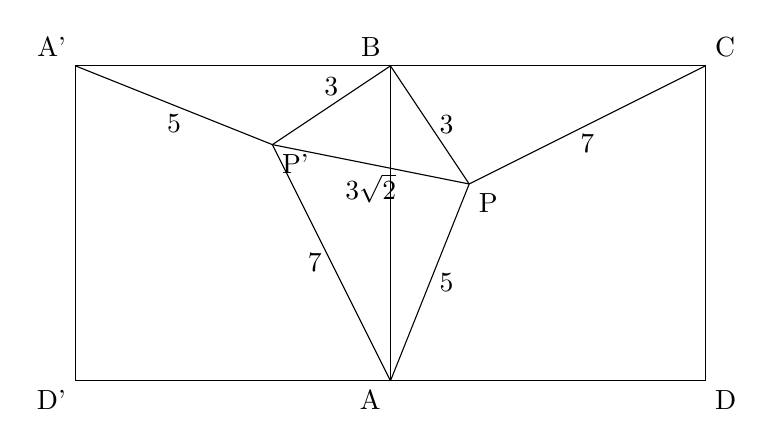
\begin{tikzpicture}
        \draw (0,0) -- (0,4) -- (4,4) -- (4,0) -- cycle;
        \draw (0,0) -- (0,4) -- (-4,4) -- (-4,0) -- cycle;
        \draw (0,0) -- (1,2.5) node[right, midway]{5};
        \draw (0,4) -- (1,2.5) node[midway, right]{3};
        \draw (4,4) -- (1,2.5) node[midway, below]{7};
        \draw (-4,4) -- (-1.5,3) node[below, midway]{5};
        \draw (0,4) -- (-1.5,3) node[midway, above]{3};
        \draw (0,0) -- (-1.5,3) node[midway, left]{7};
        \draw (-1.5,3) -- (1, 2.5) node[midway, below]{$3\sqrt{2}$};
        \node[below left] at (0,0) {A};
        \node[above left] at (0,4) {B};
        \node[above right] at (4,4) {C};
        \node[below right] at (4,0) {D};
        \node[above left] at (-4,4) {A'};
        \node[below left] at (-4,0) {D'};
        \node[below right] at (1,2.5) {P};
        \node[below right] at (-1.5, 3) {P'};
    \end{tikzpicture}
    
    where $B'=B$ and $C'=A$. Then $|\angle P'BP| = \frac{\pi}{2}$ and $|PP'| = 3\sqrt{2}$. We can apply the cosine rule for the triangle $AP'P$ to find the angle $\angle AP'P$ with:
    \[ \cos(\angle AP'P) = \frac{7^2 + (3\sqrt{2})^2 - 5^2}{2(7)(3\sqrt{2})} = \frac{1}{\sqrt{2}} \]
    
    So $\angle AP'P = \angle BP'P = \frac{\pi}{4}$ and
    \[ s^2 = 3^2 + 7^2 = 58 \]
    by Pythagoras's theorem, and the side length of the square is $\sqrt{58}$.
    
    \item Let $f(x)$ be a function such that $f(1) = 1$ and, for $x \geq 1$
    \[f'(x) = \frac{1}{x^2+f^2(x)}\]
    Prove that \[\lim_{x \to \infty} f(x)\] exists and is less than $1 + \frac{\pi}{4}$.
    
    \textbf{Answer:} Note that $f'(x) > 0$ for all $x \in \mathbb{R}$, so $f$ is strictly increasing, and since $f(1)=1$, we have $f(x)> 1$ for $x \in (1,\infty)$.
    
    \begin{align*}
         f(x)-f(1) & = \int_1^x f'(t) dt \\
         & = \int_1^x \frac{1}{t^2 + f^2(t)} dt \\
         & < \int_1^x \frac{1}{t^2+1} dt \\
         & = \tan^{-1}(x) - \tan^{-1}(1) \\
         f(x) &< 1 - \frac{\pi}{4} + \tan^{-1}(x)
    \end{align*}
    for all $x \in (1,\infty)$.
    
    Taking limits for $x$ to $\infty$ on both sides, we get
\[ \lim_{x \to \infty} f(x) < 1 - \frac{\pi}{4} + \lim_{x \to \infty} \tan^{-1} (x) = 1 + \frac{\pi}{4} \]
    
    
    \item Prove that the number of odd binomial coefficients in each row of Pascal's Triangle is a power of 2. (In Pascal's Triangle, 
    \begin{center}
    \begin{tabular}{ccccccccc}
    &    &    &    &  1\\\noalign{\smallskip\smallskip}
    &    &    &  1 &    &  1\\\noalign{\smallskip\smallskip}
    &    &  1 &    &  2 &    &  1\\\noalign{\smallskip\smallskip}
    &  1 &    &  3 &    &  3 &    &  1\\\noalign{\smallskip\smallskip}
    \end{tabular}
    \end{center}
    each entry is the sum of the entries directly above it, with the first and last entries of each row being 1.)
    
    \textbf{Answer:} The binomial coefficients $\binom{2^n}{k}$ are even for all $1 \leq k \leq 2^n-1$, since the power of 2 that divides $2^n!$ is 
    \begin{align*}
    \lfloor \frac{2^n}{2} \rfloor + \lfloor \frac{2^n}{2^2} \rfloor + \lfloor \frac{2^n}{2^3} \rfloor + \cdots & = 2^{n-1} + 2^{n-2} + \cdots + 2 + 1 \\
    &= 2^n - 1
    \end{align*}
    and the power of 2 which divides $k!(2^n-k)!$ will always be less than the power of 2 in $2^{n-1}!2^{n-1}!$, which is
    \begin{align*}
        2 \left( \lfloor \frac{2^{n-1}}{2} \rfloor + \lfloor \frac{2^{n-1}}{2^2} \rfloor + \cdots + \right)  &= 2(2^{n-2} + 2^{n-3} + \cdots + 1) \\
        &= 2^{n-1}-2
    \end{align*}
    
    so every binomial coefficient (other than $\binom{2^n}{0}$ and $\binom{s^2}{2^n}$) is even.
    
    That means $(1+x)^{2^n} \equiv 1+x^{2^n} \pmod{2}$ so for an arbitrary $m$, we can use the binary decomposition of $m = 2^{a_0} + 2^{a_1} + 2^{a_2} + \cdots$ to get:
    \begin{align*}
        (1+x)^m &= (1+x)^{2^{a_0}}(1+x)^{2^{a_1}}(1+x)^{2^{a_2}}\cdots \\
        & \equiv (1+x^{2^{a_0}})((1+x^{2^{a_1}})(1+x^{2^{a_2}})\cdots \pmod{2}
    \end{align*}
    This is an expression with a number of binomials equal to the number of 1s in the binary representation of $m$, each of the sums of the powers of 2 in the product will be distinct, and so the product will include $2^{b(m)}$ terms, where $b(m)$ is the number of 1s in the binary representation of $m$. In summary, the binomial expansion of $(1+x)^m \pmod{2}$ will have $2^{b(m)}$ terms, and there are $2^{b(m)}$ odd binomal coefficients in the $m$th row of Pascal's triangle.
    
\end{enumerate}

\end{document}


